\chapter{Analyse Réseau avec Suricata}

\section{Déploiement de Suricata}

\subsection{Architecture de détection}

Suricata v7.0~\cite{suricata_mqtt} est déployé en mode \textbf{IDS passif} (lecture uniquement, sans blocage) sur le segment réseau Services. Le trafic est dupliqué vers Suricata via un switch GNS3 configuré en mode hub, ce qui permet d'inspecter tous les paquets sans perturber le flux nominal.

Le diagramme d'activité de la figure~\ref{fig:suricata_detection} illustre le processus de détection de Suricata, depuis la capture des paquets jusqu'à la génération des alertes.

\begin{figure}[H]
  \centering
  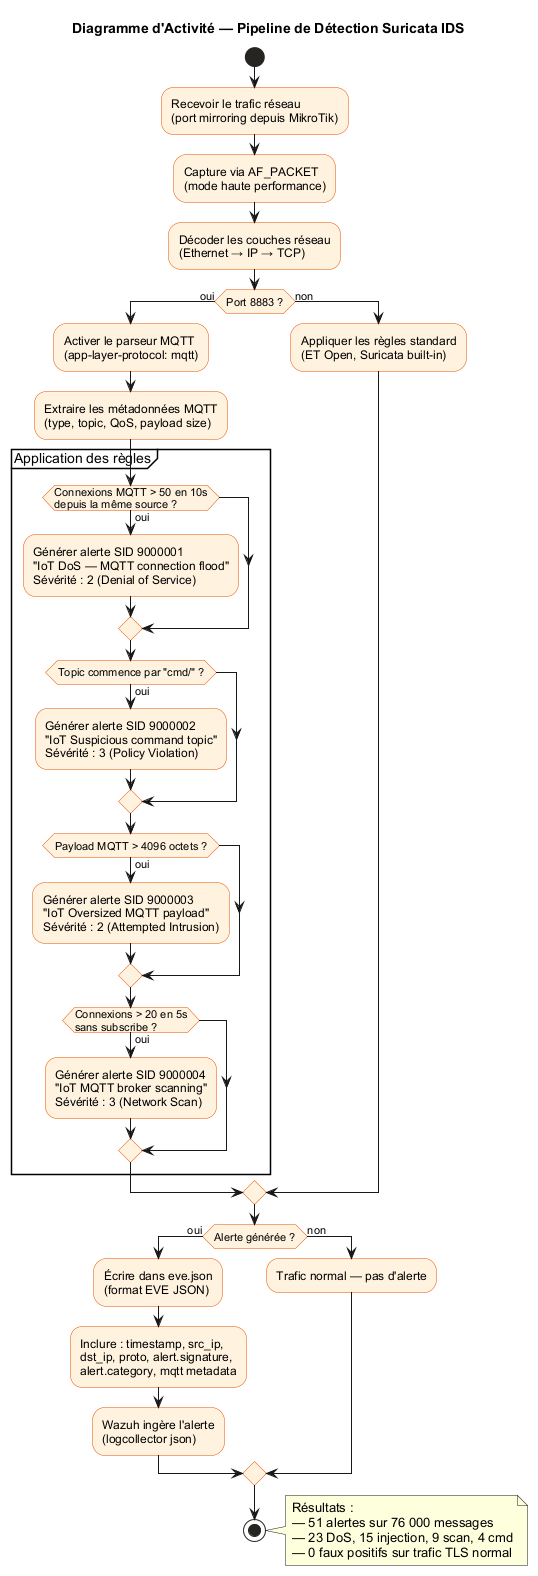
\includegraphics[width=0.8\textwidth]{diagrams/diag-suricata-detection.png}
  \caption{Processus de détection Suricata -- diagramme d'activité}
  \label{fig:suricata_detection}
\end{figure}

\subsection{Mode de capture}

Suricata utilise le mode \textbf{AF\_PACKET} pour la capture haute performance, avec les paramètres suivants :
\begin{itemize}
  \item Interface : \texttt{eth0} (segment Services).
  \item Cluster ID : 99 (mode \texttt{cluster\_flow} pour la répartition multi-thread).
  \item Défragmentation activée.
  \item Ring buffer de 2048 entrées avec \texttt{mmap} activé.
\end{itemize}

\subsection{Activation du décodeur MQTT}

Depuis Suricata 6.0, le protocole MQTT est supporté nativement via le moteur d'analyse applicative. Le décodeur est activé dans la configuration \texttt{suricata.yaml} avec une taille maximale de message de 1~Mo. La configuration complète est fournie en Annexe~B (section~\ref{sec:config_suricata}).

\section{Règles de détection personnalisées}

Quatre règles personnalisées ont été développées pour détecter les typologies d'attaques du dataset. Le tableau~\ref{tab:regles_suricata} résume ces règles.

\begin{table}[H]
\centering
\caption{Règles Suricata personnalisées pour la détection des attaques IoT}
\label{tab:regles_suricata}
\begin{tabular}{clp{4.5cm}l}
\toprule
\textbf{SID} & \textbf{Nom} & \textbf{Logique de détection} & \textbf{Attaque ciblée} \\
\midrule
9000001 & MQTT connection flood & Seuil de 50 connexions MQTT en 10~s depuis une même source & DoS \\
9000002 & Suspicious cmd topic & Publication sur un topic commençant par \texttt{cmd/} & MiTM / Replay \\
9000003 & Oversized payload & Payload MQTT de plus de 4096~octets & Injection \\
9000004 & Broker scanning & 20+ connexions en 5~s sans souscription & Scanning \\
\bottomrule
\end{tabular}
\end{table}

Les règles utilisent les mots-clés Suricata spécifiques au protocole MQTT : \texttt{mqtt.type} (type de paquet MQTT), \texttt{mqtt.topic} (filtrage par topic) et \texttt{dsize} (taille du payload). Le texte complet des règles est fourni en Annexe~B.

\section{Analyse des alertes}

\subsection{Volume d'alertes générées}

Suricata a généré \textbf{51 alertes} au total sur la durée de la simulation. La distribution par règle est la suivante :

\begin{table}[H]
\centering
\caption{Distribution des alertes Suricata par règle}
\label{tab:suricata_alerts}
\begin{tabular}{llrl}
\toprule
\textbf{SID} & \textbf{Description} & \textbf{Alertes} & \textbf{Type d'attaque} \\
\midrule
9000001 & MQTT connection flood & 23 & DoS \\
9000003 & Oversized payload & 15 & FalsifiedData / Injection \\
9000004 & Broker scanning & 9 & Scanning \\
9000002 & Suspicious cmd topic & 4 & MiTM / Replay \\
\midrule
 & \textbf{Total} & \textbf{51} & \\
\bottomrule
\end{tabular}
\end{table}

\subsection{Format des alertes EVE JSON}

Suricata génère ses alertes dans le format \textbf{EVE JSON} (\texttt{/var/log/suricata/eve.json}), qui est directement ingérable par Wazuh. Chaque alerte contient les informations suivantes :
\begin{itemize}
  \item \textbf{Horodatage} avec précision à la microseconde.
  \item \textbf{Adresses source et destination} (IP et port).
  \item \textbf{Protocole applicatif} détecté (\texttt{mqtt}).
  \item \textbf{Détails de l'alerte} : signature, catégorie, sévérité.
  \item \textbf{Métadonnées MQTT} : type de paquet, QoS, identifiant.
\end{itemize}

Un exemple d'alerte EVE JSON est fourni en Annexe~B.

\begin{figure}[H]
  \centering
  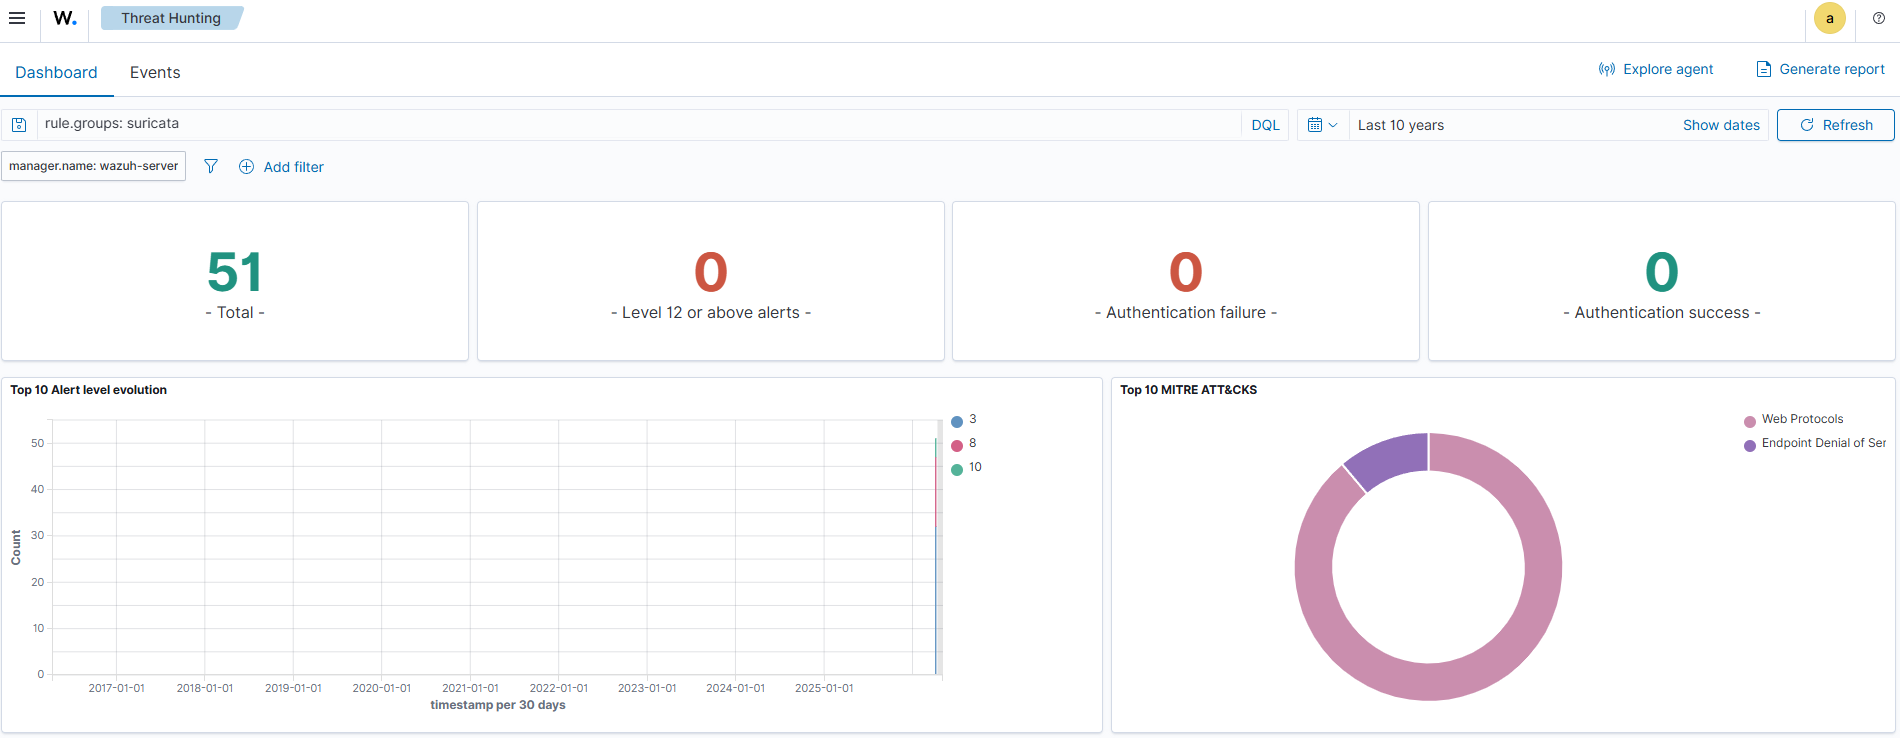
\includegraphics[width=\textwidth]{figures/suricata-alerts.png}
  \caption{Alertes Suricata visibles dans le dashboard Wazuh}
  \label{fig:suricata_wazuh}
\end{figure}

\begin{resultbox}[Résultats Suricata]
\textbf{51 alertes} générées sur 76\,000 messages. Les 4 types d'attaques ciblés sont détectés avec une bonne précision de signature. Aucun faux-positif sur le trafic normal TLS.
\end{resultbox}
